\documentclass[t,11pt]{beamer}

\usepackage[francais]{babel}
\usepackage[T1]{fontenc}
\usepackage[utf8]{inputenc}
\usepackage{hyperref}

\usetheme{Warsaw}
\setbeamercolor{background canvas}{bg=yellow!10!white}


\title{Introduction pragmatique à Git}
\author{K\'evin Unger\hspace{1mm} \newline kevin.unger@fresnel.fr}
\institute
{
        Institut Fresnel\\
        \url{https://github.com/kevung/git-presentation.git}
}
\date{\today}

\begin{document}

%----------------------------------------------
\begin{frame}[plain,c]
        \titlepage
\end{frame}

%----------------------------------------------
%table des matieres
\begin{frame}[c]
        \frametitle{Sommaire}
        \tableofcontents[hideallsubsections]
\end{frame}

%----------------------------------------------
%table des matieres auto a chaque section
\AtBeginSection[]{
\begin{frame}[c]
        \tableofcontents[currentsection,hideallsubsections]
\end{frame}
}

%----------------------------------------------
\section{Git?! A quoi ça sert\ldots}


\subsection{Situation n. 1}
\begin{frame}[label=sit1]
        \frametitle{Situation n. 1}
        \framesubtitle{Comment garder des traces sans perdre la tête?}
        \vspace{-2mm}
        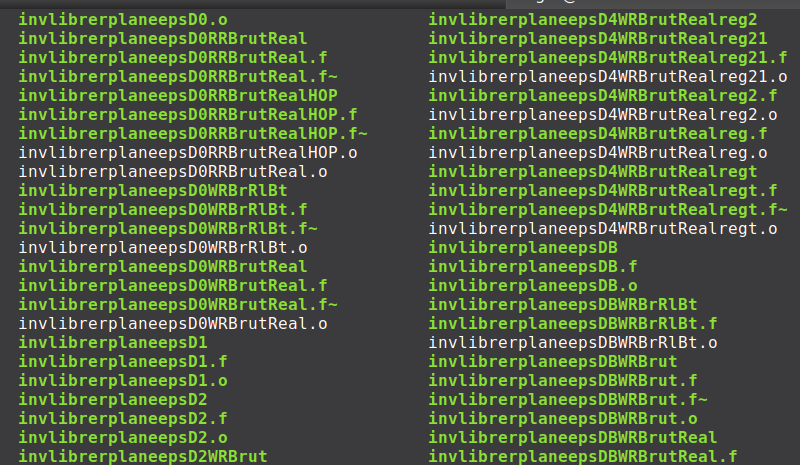
\includegraphics[width=\linewidth]{./img/bazar_crop2}
\end{frame}


\subsection{Situation n. 2}
\begin{frame}[label=sit2]
        \frametitle{Situation n. 2}
        \framesubtitle{Comment tester sans avoir peur de tout casser?}
        \begin{center}
                \vspace{-5mm}
        
\includegraphics[width=\linewidth,height=0.8\textheight,keepaspectratio]{./img/debugging}
        \end{center}
\end{frame}


\subsection{Situation n. 3}
%\begin{frame}[label=sit3,fragile,c]
\begin{frame}[label=sit3,c]
        \frametitle{Situation n. 3}
        \framesubtitle{Comment travailler simultane\'ment sur un même document?}
        \begin{semiverbatim}
        \begin{itemize}
                \item[1)] C'est toi qui a la dernière version de la biblio?
                \item[2)] Oui, je l'ai modifiée hier, mais je te l'ai envoyée par mail. 
                \item[1)] Zut, j'ai aussi travaillé dessus\ldots
                \item[1)] C'est \texttt{bib10051788\_v2corigee\_NewNew.bib}?
        \end{itemize}
        \end{semiverbatim}
\end{frame}

%----------------------------------------------
\section{Garder des traces proprement}

\subsection{Principe}
\begin{frame}[c]
        \frametitle{Principe}
        \begin{columns}
                \column{0.5\linewidth}
                \begin{block}{Cr\'ee un d\'ep\^ot Git}
                        \centering
                        git init
                \end{block}
        \end{columns}
        \begin{center}
                \hspace{1.1cm}
                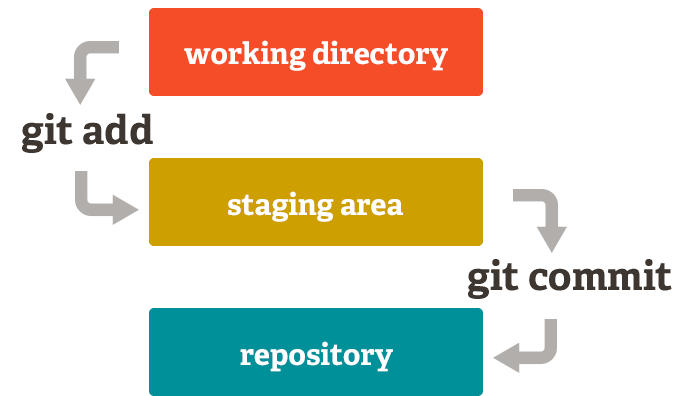
\includegraphics[width=0.5\linewidth]{./img/git_staging_area}
                \newline
                \hspace*{15pt}
                \href{https://git-scm.com/about/staging-area}{{\tiny (source: Pro Git)}}
        \end{center}
\end{frame}

\subsection{Versionnage du projet}
\begin{frame}[c]
        \frametitle{Versionnage du projet}
        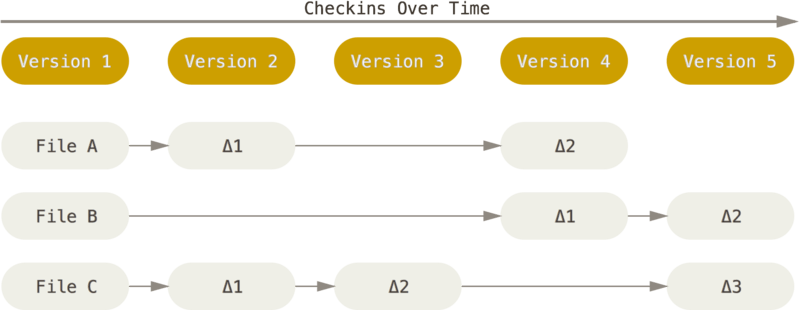
\includegraphics[width=\linewidth]{./img/deltas}
        \newline
        \hspace*{15pt}
        \href{https://git-scm.com/book/fr/v2/D\%C3\%A9marrage-rapide-Rudiments-de-Git}{{\tiny (source: Pro Git)}}
\end{frame}

%\subsection{Cycle de vie d'un fichier}
%\begin{frame}[c]
%        \frametitle{Cycle de vie d'un fichier}
%        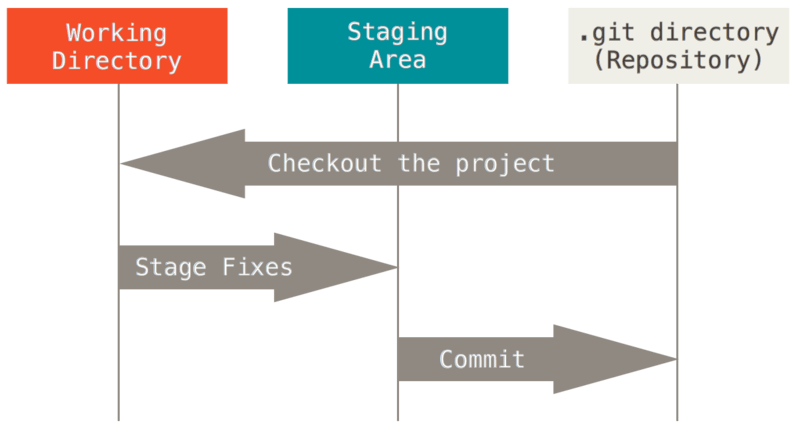
\includegraphics[width=\linewidth]{./img/git_cycle}
%        \newline
%        \hspace*{15pt}
%        \href{https://git-scm.com/book/fr/v2/Les-bases-de-Git-Enregistrer-des-modifications-dans-le-d\%C3\%A9p\%C3\%B4t}{{\tiny (source: Pro Git)}}
%\end{frame}


\subsection{Exemple d'historique}
\begin{frame}[c]
        \frametitle{Exemple d'historique}
        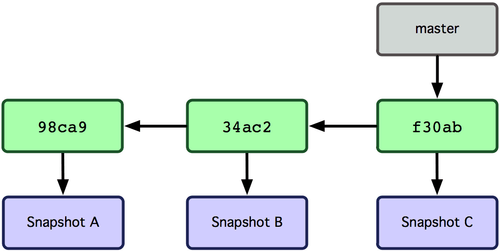
\includegraphics[width=\linewidth]{./img/master_branch}
        \newline
        \hspace*{15pt}
        \href{https://git-scm.com/book/fr/v1/Les-branches-avec-Git-Ce-qu-est-une-branche}{{\tiny (source: Pro Git)}}
\end{frame}

\subsection{Cinq commandes}
\begin{frame}[t]
        \frametitle{Cinq commandes}
        \begin{columns}
                \column{0.5\linewidth}
                \begin{block}{Affiche l'\'etat du d\'ep\^ot}
                        \centering
                        git status
                \end{block}
        \end{columns}

        \begin{columns}
                \column{0.5\linewidth}
                \begin{block}{Ajoute pour le prochain archivage}
                        \centering
                        git add
                \end{block}
                \column{0.5\linewidth}

                \begin{block}{Archive}
                        \centering
                        git commit
                \end{block}
        \end{columns}

        \begin{columns}
                \column{0.5\linewidth}
                \begin{block}{Affiche l'historique}
                        \centering
                        git log
                \end{block}

                \column{0.5\linewidth}
                \begin{block}{Restaure l'\'etat d'une archive}
                        \centering
                        git checkout \emph{mon-commit}
                \end{block}
        \end{columns}
\end{frame}

%----------------------------------------------
\section{Exp\'erimenter en toute s\'er\'enit\'e}

\subsection{Cr\'eer des branches}

\begin{frame}
        \frametitle{Cr\'eer des branches}
        \centering
        \hspace{10mm}
        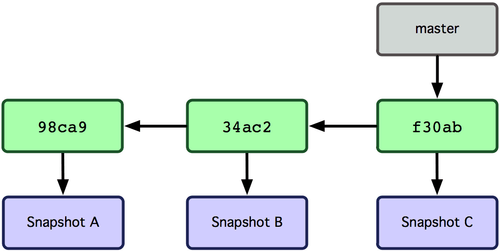
\includegraphics[width=\linewidth,height=0.4\textheight,keepaspectratio]{./img/branching_1}
        \newline
        \href{https://git-scm.com/book/fr/v1/Les-branches-avec-Git-Ce-qu-est-une-branche}{{\tiny (source: Pro Git)}}
        \begin{columns}
                \column{0.5\linewidth}
                \begin{block}{Cr\'eer une branche}
                        \centering
                        git branch \emph{ma-nouvelle-branche}
                \end{block}
        \end{columns}
\end{frame}

\begin{frame}
        \frametitle{Cr\'eer des branches}
        \centering
        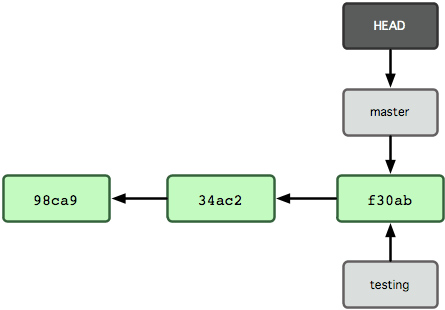
\includegraphics[width=\linewidth,height=0.8\textheight,keepaspectratio]{./img/branching_2}
        \newline
        \href{https://git-scm.com/book/fr/v1/Les-branches-avec-Git-Ce-qu-est-une-branche}{{\tiny (source: Pro Git)}}
\end{frame}

\begin{frame}
        \frametitle{Cr\'eer des branches}
        \centering
        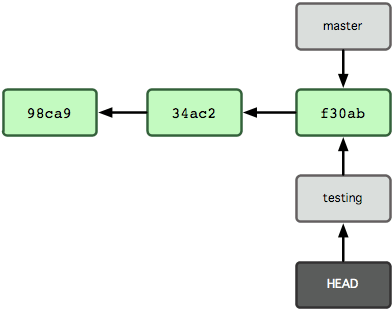
\includegraphics[width=\linewidth,height=0.8\textheight,keepaspectratio]{./img/branching_3}
        \newline
        \href{https://git-scm.com/book/fr/v1/Les-branches-avec-Git-Ce-qu-est-une-branche}{{\tiny (source: Pro Git)}}
\end{frame}

\begin{frame}
        \frametitle{Cr\'eer des branches}
        \centering
        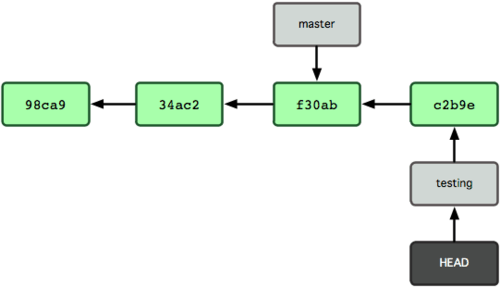
\includegraphics[width=\linewidth,height=0.8\textheight,keepaspectratio]{./img/branching_4}
        \newline
        \href{https://git-scm.com/book/fr/v1/Les-branches-avec-Git-Ce-qu-est-une-branche}{{\tiny (source: Pro Git)}}
\end{frame}

\begin{frame}
        \frametitle{Cr\'eer des branches}
        \centering
        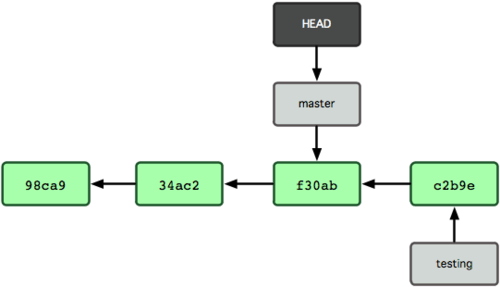
\includegraphics[width=\linewidth,height=0.8\textheight,keepaspectratio]{./img/branching_5}
        \newline
        \href{https://git-scm.com/book/fr/v1/Les-branches-avec-Git-Ce-qu-est-une-branche}{{\tiny (source: Pro Git)}}
\end{frame}

\begin{frame}
        \frametitle{Cr\'eer des branches}
        \centering
        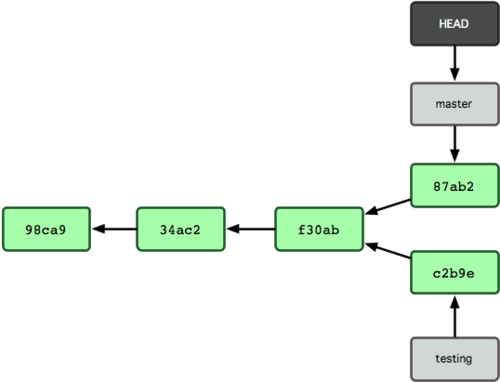
\includegraphics[width=\linewidth,height=0.8\textheight,keepaspectratio]{./img/branching_6}
        \newline
        \href{https://git-scm.com/book/fr/v1/Les-branches-avec-Git-Ce-qu-est-une-branche}{{\tiny (source: Pro Git)}}
\end{frame}


\subsection{Fusionner des branches}

\begin{frame}
        \frametitle{Fusionner des branches}
        \centering
        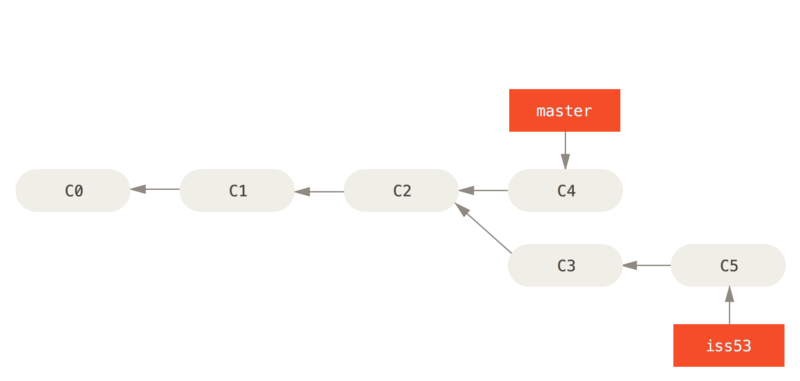
\includegraphics[width=\linewidth,height=0.8\textheight,keepaspectratio]{./img/basic-branching-6}
        \newline
        \href{https://git-scm.com/book/fr/v1/Les-branches-avec-Git-Ce-qu-est-une-branche}{{\tiny (source: Pro Git)}}
\end{frame}

\begin{frame}
        \frametitle{Fusionner des branches}
        \begin{columns}
                \column{.6\linewidth}
                \begin{block}{Fusionner dans la branche courante}
                        git merge \emph{iss53}
                \end{block}
        \end{columns}
        \vspace{-5mm}
        \centering
        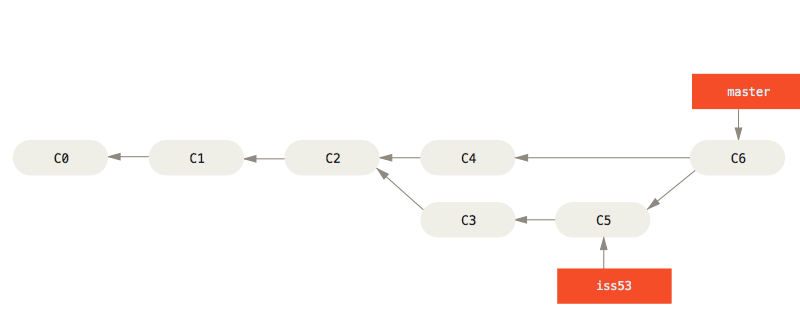
\includegraphics[width=\linewidth,height=0.8\textheight,keepaspectratio]{./img/basic-merging-2}
        \newline
        \href{https://git-scm.com/book/fr/v1/Les-branches-avec-Git-Ce-qu-est-une-branche}{{\tiny (source: Pro Git)}}
\end{frame}

\subsection{Branching model}
\begin{frame}
        \frametitle{Branching model}
        \centering
        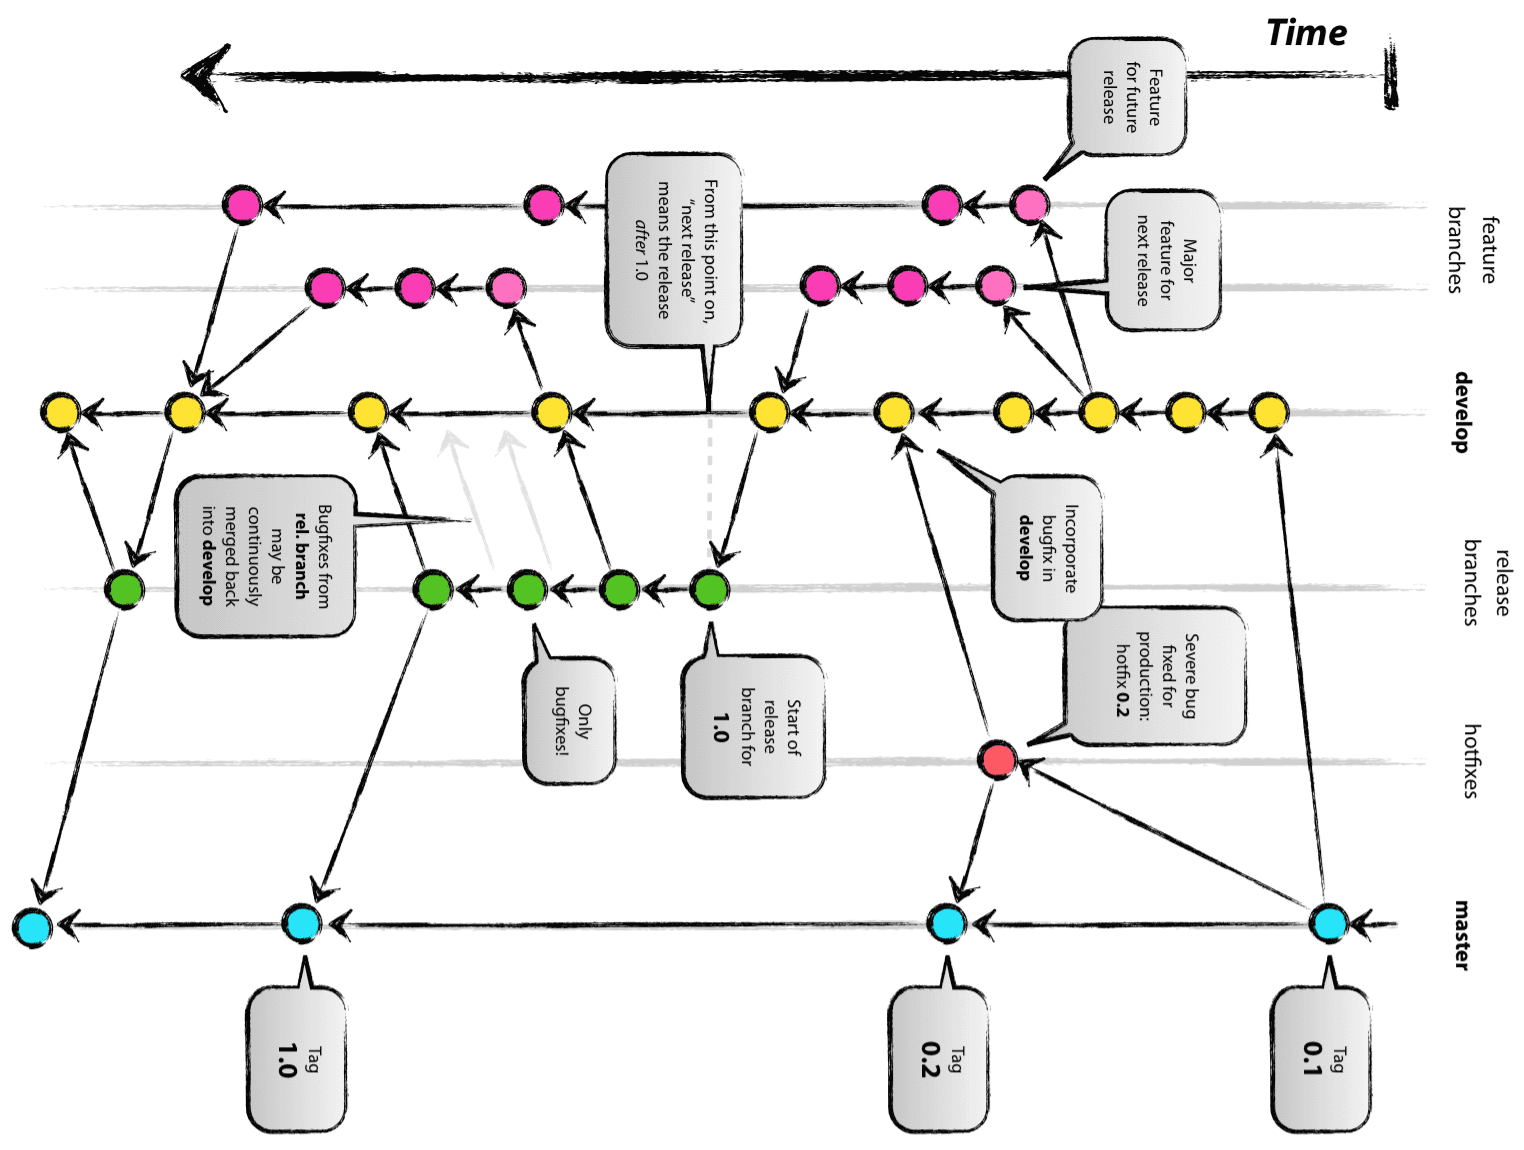
\includegraphics[width=\linewidth,height=0.8\textheight,keepaspectratio]{./img/branching_model}
        \newline
        \href{http://nvie.com/posts/a-successful-git-branching-model/}{{\tiny (http://nvie.com/posts/a-successful-git-branching-model/)}}
\end{frame}

\subsection{4 commandes}
\begin{frame}
        \frametitle{4 commandes}

        \begin{columns}
                \column{0.5\linewidth}

                \begin{block}{Créer une branche}
                        git branch \emph{ma-nouvelle-branche}
                \end{block}

                \begin{block}{Basculer sur une branche}
                        git checkout \emph{branche-cible}
                \end{block}

                \column{0.5\linewidth}

                \begin{block}{Afficher la branche courante}
                        git branch
                \end{block}

                \begin{block}{Fusionner une branche dans la branche courante}
                        git merge \emph{branche-cible}
                \end{block}

        \end{columns}

\end{frame}

%----------------------------------------------
\section{Travailler \`a plusieurs (simultan\'ement) }

\subsection{D\'ep\^ot centralis\'e}

\begin{frame}
        \frametitle{D\'ep\^ot centralis\'e}
        \centering
        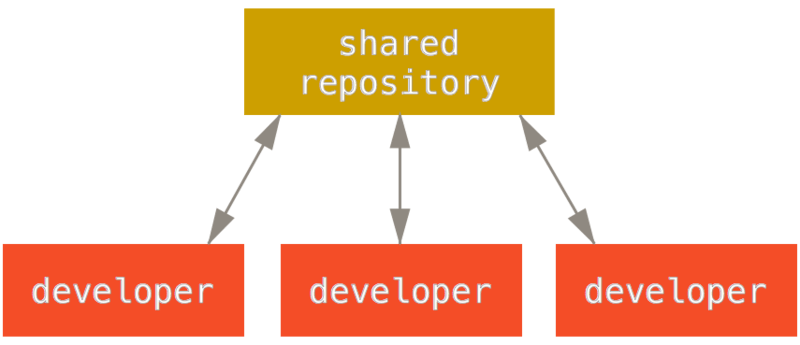
\includegraphics[width=\linewidth,height=0.8\textheight,keepaspectratio]{./img/centralized_workflow}
        \begin{block}{Cr\'eer un d\'ep\^ot vierge}
                git init --bare \emph{mon-depot.git}
        \end{block}
\end{frame}

\subsection{Trois commandes}

\begin{frame}
        \frametitle{Trois commandes}
        \begin{block}{Ajouter l'adresse d'un d\'ep\^ot distant}
                git remote add \emph{mon-depot} \emph{adresse-de-mon-depot}
        \end{block}
        \begin{block}{Pousser sur un d\'ep\^ot distant}
                git push \emph{mon-depot} \emph{branche-sur-mon-depot}
        \end{block}
        \begin{block}{Tirer sur un d\'ep\^ot distant}
                git pull \emph{mon-depot} \emph{branche-sur-mon-depot}
        \end{block}
\end{frame}

%-----------------------------------------------
\appendix
\begin{frame}[c]
        \frametitle{Annexes}
        \tableofcontents[hideallsubsections]
\end{frame}

%-----------------------------------------------
\section{Configurer Git}
\subsection{Configuration initiale}
\begin{frame}
        \frametitle{Configuration initiale}
        \begin{block}{Identit\'e}
                git config --global user.name "\emph{Augustin Fresnel}"
        \end{block}
        
        \begin{block}{Email}
                git config --global user.email "\emph{augustin.fresnel@fresnel.fr}"
        \end{block}

        \begin{block}{Editeur}
                git config --global core.editor \emph{emacs}
        \end{block}
\end{frame}

\subsection{Les alias}
\begin{frame}
        \frametitle{Les alias}
        \vspace{-7mm}
        \begin{columns}
                \column{0.6\linewidth}

                \begin{block}{checkout -> co}
                        git config --global alias.\emph{co} checkout
                \end{block}

                \begin{block}{branch -> br}
                        git config --global alias.\emph{br} branch
                \end{block}

                \begin{block}{status -> st}
                        git config --global alias.\emph{st} status
                \end{block}

                \begin{block}{commit -> ci}
                        git config --global alias.\emph{ci} commit
                \end{block}

        \end{columns}
\end{frame}

%-----------------------------------------------
\section{Explorer l'historique}
\subsection{git difftool}
\begin{frame}
        \frametitle{git difftool \emph{commit-1} \emph{commit-2}}
        \centering
        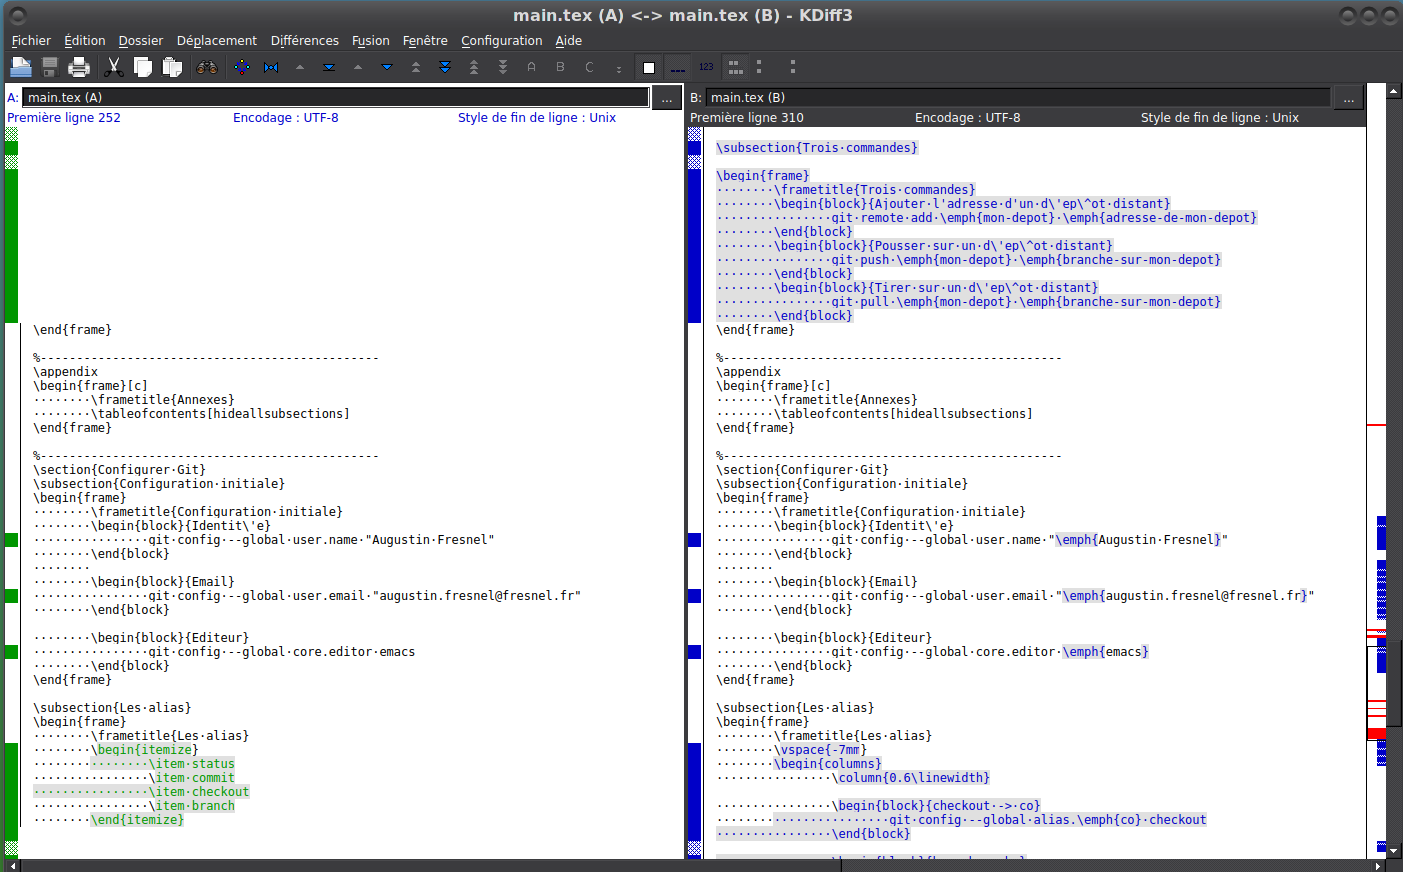
\includegraphics[width=\linewidth,height=0.8\textheight,keepaspectratio]{./img/git-difftool-kdiff3.png}
\end{frame}

\subsection{Interfaces Git graphiques}
\begin{frame}
        \frametitle{Interfaces Git graphiques}
\end{frame}


%-----------------------------------------------
\section{G\'erer les conflits de fusion}
\subsection{git mergetool}
\begin{frame}
        \frametitle{git mergetool}
        \centering
        \vspace{8mm}
        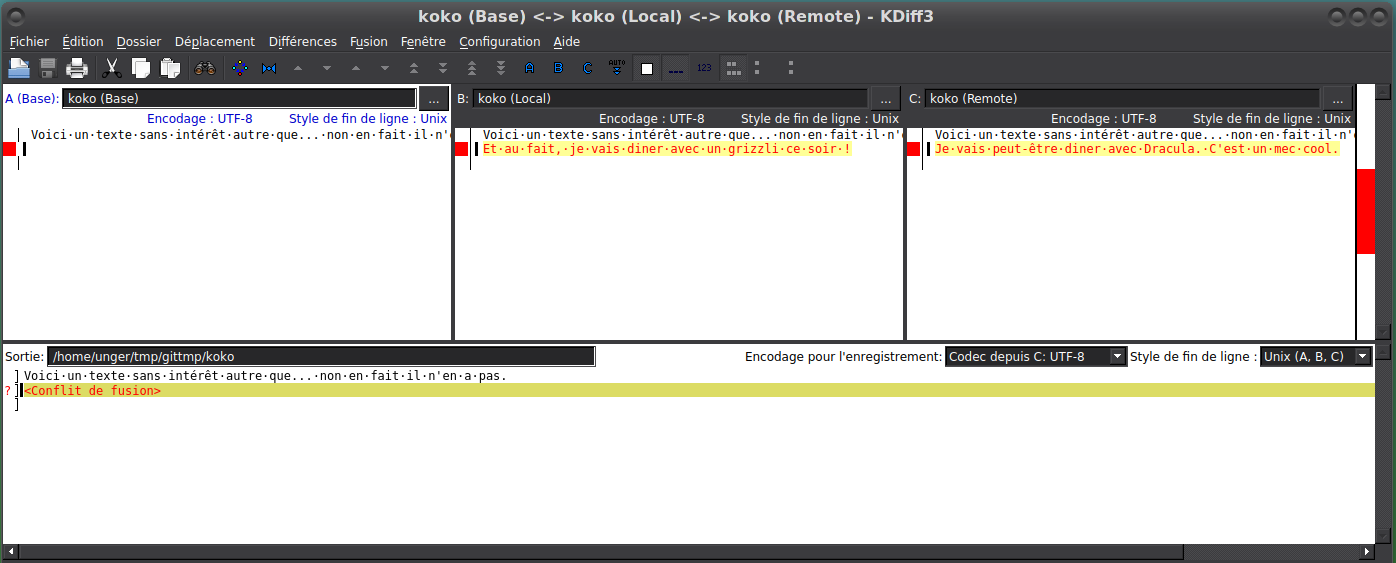
\includegraphics[width=\linewidth,height=\textheight,keepaspectratio]{./img/git-mergetool-kdiff3.png}
\end{frame}

\section{Travailler sur plusieurs branches}
\subsection{git stash}
\begin{frame}
        \frametitle{git stash}
\end{frame}

\subsection{git cherry-pick}
\begin{frame}
        \frametitle{git cherry-pick}
\end{frame}

%-----------------------------------------------
\section{Int\'egration avec le shell}
\begin{frame}
        \frametitle{Int\'egration avec le shell}
        zsh + oh-my-zsh + plugin git
\end{frame}

%-----------------------------------------------
\section{Bibliographie}
\begin{frame}
        \frametitle{Bibliographie}
\end{frame}
\end{document}
